% Roads & Realms: das Handbuch (deutsch). Bauen: manual/build.sh de (pdfLaTeX)
\documentclass[a4paper,11pt,oneside,DIV=12,headings=small,toc=chapterentrydotfill]{scrbook}
\usepackage[ngerman]{babel}
% The manual's look: the game's own colours (wood, parchment, gold), framed screenshots,
% building cards. Shared by every language's book.
% (pdfLaTeX and the TeX tree's own fonts: this machine's LuaTeX has no font loader)
\usepackage[T1]{fontenc}
\usepackage[utf8]{inputenc}
\usepackage{textcomp}
\usepackage{tgpagella}
\usepackage[scale=0.92]{tgheros}
\providecommand{\rrhead}{\normalfont\rmfamily}
\providecommand{\rrtitle}{\normalfont\rmfamily}
\DeclareUnicodeCharacter{2212}{\textminus}
\DeclareUnicodeCharacter{00D7}{\texttimes}
\DeclareUnicodeCharacter{2716}{$\times$}
\DeclareUnicodeCharacter{2192}{$\rightarrow$}
\DeclareUnicodeCharacter{2606}{$\star$}
\DeclareUnicodeCharacter{2693}{\textsf{Anker}}
\DeclareUnicodeCharacter{2605}{$\bigstar$}
\usepackage{csquotes}

\usepackage{xcolor}
\definecolor{paper}{HTML}{FBF6EA}
\definecolor{paperdark}{HTML}{F1E6CF}
\definecolor{wood}{HTML}{40301E}
\definecolor{woodmid}{HTML}{6B4A2A}
\definecolor{gold}{HTML}{B8862F}
\definecolor{goldlight}{HTML}{E9C77E}
\definecolor{ink}{HTML}{2A2118}
\definecolor{leaf}{HTML}{4F7A34}
\pagecolor{paper}
\color{ink}

\usepackage{graphicx}
\usepackage{array,booktabs,tabularx}
\usepackage{enumitem}
\setlist{itemsep=2pt,topsep=4pt}
\setlist[itemize]{label={\color{gold}\small$\blacktriangleright$}}
\usepackage{amssymb}
\usepackage{microtype}
\usepackage{tikz}
\usetikzlibrary{positioning,shadows.blur,calc,arrows.meta,fit,backgrounds,fadings,chains}
\tikzset{bld/.style={draw=wood, fill=paperdark, rounded corners=2pt, inner sep=3pt, font=\sffamily\small},
  ware/.style={fill=goldlight!70, rounded corners=7pt, inner sep=3pt, font=\sffamily\small},
  s/.style={fill=wood, text=goldlight, rounded corners=2pt, inner sep=3pt, font=\sffamily\small\bfseries},
  b/.style={bld, text height=1.6ex, text depth=0.45ex}, w/.style={ware, text height=1.6ex, text depth=0.45ex},
  s/.append style={text height=1.6ex, text depth=0.45ex}}
% \chain{b/Förster, w/Bäume, ...}: buildings and wares in a row, joined by arrows
\newcommand{\chain}[1]{\tikz[baseline=(c-1.base), start chain=c going right, node distance=4.5mm,
  every join/.style={-{Stealth[length=4pt]}, woodmid, line width=0.7pt}]{%
  \foreach \t/\n [count=\i] in {#1}{\ifnum\i=1 \node[\t, on chain]{\n};\else\node[\t, on chain, join]{\n};\fi}}}
\usepackage[most]{tcolorbox}
\usepackage{needspace}
\usepackage[hidelinks]{hyperref}
\hypersetup{pdfauthor={Roads \& Realms}}

% headings in the title's serif and the windows' gold-brown
\setkomafont{disposition}{\rrhead\color{wood}}
\setkomafont{chapter}{\Huge}
\setkomafont{section}{\LARGE}
\setkomafont{subsection}{\Large}
\setkomafont{chapterentry}{\rrhead\color{wood}}
\renewcommand*{\chapterformat}{%
  \textcolor{gold}{\fontsize{44}{44}\selectfont\thechapter}\hspace{0.5em}}
\renewcommand*{\chapterlinesformat}[3]{%
  \parbox[b]{\linewidth}{#2#3\par\vspace{2pt}{\color{gold}\rule{\linewidth}{1.2pt}}}}
\RedeclareSectionCommand[beforeskip=-1.6\baselineskip,afterskip=0.6\baselineskip]{section}
% a heading never stands alone at the foot of a page, above a picture that moved on
\AddToHook{cmd/section/before}{\needspace{16\baselineskip}}

\usepackage[headsepline=0.4pt:,footsepline=0pt]{scrlayer-scrpage}
\pagestyle{scrheadings}
\automark[chapter]{chapter}
\clearpairofpagestyles
\ihead{\sffamily\footnotesize\color{woodmid}Roads \& Realms}
\ohead{\sffamily\footnotesize\color{woodmid}\leftmark}
\cfoot{\sffamily\small\color{woodmid}\pagemark}
\renewcommand*{\chaptermarkformat}{}
\addtokomafont{headsepline}{\color{goldlight}}

\setlength{\parskip}{0.45\baselineskip}
\setlength{\parindent}{0pt}

% ---------------------------------------------------------------- screenshots
% \shot[width]{file}: a screenshot with rounded corners, a wooden frame and a soft shadow
\newcommand{\shot}[2][\linewidth]{%
  \begin{tikzpicture}
    \node[inner sep=0pt, blur shadow={shadow blur steps=6, shadow xshift=1.2pt, shadow yshift=-1.6pt}]
      (i) {\includegraphics[width=#1]{#2}};
    \draw[wood, line width=1.6pt, rounded corners=3pt] (i.south west) rectangle (i.north east);
  \end{tikzpicture}}
% \screen{file}{caption}: a full-width screenshot with its caption below
\newcommand{\screen}[2]{%
  \par\needspace{\dimexpr0.54\linewidth+3\baselineskip}\begin{center}\shot[0.86\linewidth]{#1}\par\vspace{3pt}
  {\sffamily\small\color{woodmid}#2}\end{center}}
% \window{file}{width}{text}: a window cut out of the screen, beside its description
\newcommand{\window}[3]{%
  \par\noindent
  \begin{minipage}[t]{#2}\vspace{0pt}\shot{#1}\end{minipage}\hfill
  \begin{minipage}[t]{\dimexpr\linewidth-#2-1.2em}\vspace{0pt}#3\end{minipage}\par\medskip}

% ---------------------------------------------------------------- boxes
\newtcolorbox{tipbox}[1][Tipp]{enhanced, breakable, colback=paperdark, colframe=gold, boxrule=0pt,
  leftrule=3pt, arc=2pt, left=8pt, right=8pt, top=4pt, bottom=4pt,
  fonttitle=\sffamily\bfseries\small, coltitle=woodmid, title={#1}, attach title to upper={\quad},
  before skip=8pt, after skip=8pt}
\newtcolorbox{storybox}{enhanced, breakable, colback=wood, colupper=goldlight, boxrule=0pt, arc=3pt,
  left=10pt, right=10pt, top=7pt, bottom=7pt, fontupper=\itshape\small}
\newcommand{\key}[1]{\tikz[baseline=(k.base)]\node[draw=woodmid, fill=paperdark, rounded corners=2pt,
  inner sep=2pt, font=\sffamily\footnotesize, text=wood] (k) {#1};}

% ---------------------------------------------------------------- buildings
\newcommand{\fact}[2]{{\sffamily\small\color{woodmid}#1} & {\small #2}\\}
\newcommand{\tip}[1]{\par\smallskip{\sffamily\small\color{gold}\textbf{Tipp:}}~{\small #1}}
% \building{name}{picture}{facts}{text}{tip}
\newcommand{\building}[5]{%
  \begin{tcolorbox}[enhanced, breakable=false, colback=white!60!paper, colframe=wood, arc=3pt,
    boxrule=0.8pt, title={#1}, fonttitle=\rrhead\large, coltitle=goldlight, colbacktitle=wood,
    sidebyside, sidebyside align=top seam, lefthand width=3.6cm, sidebyside gap=10pt, segmentation hidden,
    left=6pt, right=8pt, top=6pt, bottom=6pt, before skip=6pt, after skip=8pt]
    \centering\includegraphics[width=\linewidth,height=3.4cm,keepaspectratio]{#2}
    \tcblower
    \begin{tabular}{@{}l>{\raggedright\arraybackslash}p{\dimexpr\linewidth-2.6cm}@{}}#3\end{tabular}\par
    \smallskip#4#5
  \end{tcolorbox}}

\graphicspath{{build/de/img/}}
\hypersetup{pdftitle={Roads \& Realms: Handbuch}}

\begin{document}

% ================================================================ Titel
\begin{titlepage}
\begin{tikzpicture}[remember picture, overlay]
  \node[inner sep=0, anchor=center] at (current page.center)
    {\includegraphics[height=\paperheight]{overview.png}};
  \fill[wood, opacity=0.55] (current page.south west) rectangle (current page.north east);
  \fill[wood, path fading=south, opacity=0.95]
    ($(current page.north west)$) rectangle ($(current page.north east)+(0,-14cm)$);
  \fill[wood, opacity=0.92] ($(current page.south west)$) rectangle ($(current page.south east)+(0,6.2cm)$);
  \node at ($(current page.north)+(0,-5.4cm)$)
    {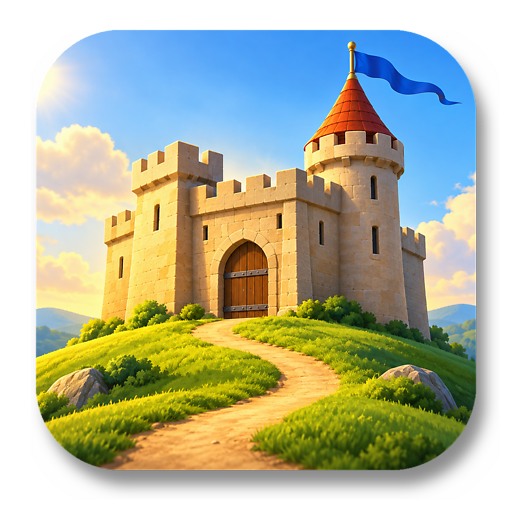
\includegraphics[width=3.4cm]{../../../assets/icon/roads-and-realms-512.png}};
  \node[text=goldlight, font=\rrtitle\fontsize{54}{58}\selectfont] at ($(current page.north)+(0,-9.4cm)$)
    {Roads \& Realms};
  \node[text=paper, font=\rrhead\itshape\LARGE] at ($(current page.north)+(0,-11cm)$)
    {bauen · tragen · erobern};
  \node[text=goldlight, font=\rrhead\Huge] at ($(current page.south)+(0,4cm)$) {Handbuch};
  \node[text=paper, font=\sffamily\large, align=center] at ($(current page.south)+(0,2.4cm)$)
    {Aufbau, Wirtschaft und Krieg · alle Gebäude · alle Fenster · die Kampagne};
\end{tikzpicture}
\end{titlepage}

\frontmatter
\tableofcontents

\mainmatter
% ================================================================ 1
\chapter{Willkommen}

\textbf{Roads \& Realms} ist ein Aufbau- und Strategiespiel. Du gründest ein Reich, baust Straßen von Fahne
zu Fahne und siehst zu, wie deine Träger jede Ware Stück für Stück an ihr Ziel bringen. Aus Holz werden Bretter,
aus Getreide Brot, aus Erz und Kohle Eisen, Schwerter und am Ende Goldmünzen. Mit deinen Soldaten schiebst
du die Grenzen hinaus, bis dir die Burgen deiner Gegner gehören.

Du befiehlst nie einem einzelnen Siedler, was er tun soll. Du stellst Gebäude hin, verbindest sie mit Straßen
und legst fest, wohin welche Waren gehen. Alles andere tun deine Leute selbst: Der Holzfäller sucht sich
seinen Baum, der Träger nimmt die nächste Ware von der Fahne, der Bauer sät und erntet. Ein gutes Reich ist
eines, in dem nichts stockt.

\screen{overview.png}{Ein Reich nach 25 Minuten: Burg, Wachstuben, Holzfäller, Bauernhöfe und ein dichtes Netz
aus Straßen. Oben rechts stehen die nächsten Schritte.}

\section*{Was dich erwartet}
\begin{itemize}
  \item eine \textbf{Weltkampagne} in sechs Missionen, vom ersten Tal über Europa und Nordamerika bis zum
    Meer in der Mitte der Erde, mit einer durchgehenden Geschichte;
  \item \textbf{freie Spiele} auf Zufallskarten in Grünland, Ödland oder Winterwelt, mit bis zu acht Spielern,
    Friedenszeit, Zeitlimit oder einem Ziel nach Land oder Münzen;
  \item eine \textbf{Wirtschaft} aus 32 Gebäuden, 31 Waren und 30 Berufen;
  \item \textbf{Militär} mit fünf Rängen, Beförderung durch Gold, Angriffen, Katapulten und Spähtürmen;
  \item \textbf{Seefahrt} mit Häfen, Schiffen und Expeditionen zu fremden Küsten;
  \item Computergegner in drei Stärken, \textbf{Netzwerkspiele} im lokalen Netz und einen \textbf{Karteneditor}.
\end{itemize}

\section*{Installation und Start}
Das Spiel läuft unter Linux. Im Quellverzeichnis startet es mit
\begin{center}\texttt{cargo run --release -p rr-app}\end{center}
und \texttt{tools/install-launcher.sh} legt es mit seinem Symbol in das Anwendungsmenü und das Dock von Ubuntu
(\texttt{--remove} nimmt es wieder heraus). In einem entpackten Paket heißt das Skript
\texttt{./install-launcher.sh}. Danach findest du das Spiel mit der Super-Taste und \enquote{Roads}.

Die Sprache folgt deinem System. Im Fenster \emph{Optionen} kannst du jederzeit zwischen Deutsch und Englisch
wechseln.

% ================================================================ 2
\chapter{Das Titelmenü}

\screen{menu.png}{Das Titelmenü: links die Kampagne und das freie Spiel, rechts Spielstände, Netzwerk,
Kartendateien, Editor und Optionen.}

\textbf{Kampagne.} \emph{Das erste Tal} ist die Lernmission; danach folgen die Europa-Mission und die
nummerierten Missionen. Darunter wählst du die Stärke der \textbf{Gegner}: Sie entscheidet in der Kampagne
auch, wie viele Gegner gegen dich Krieg führen (leicht: höchstens zwei, schwer: alle). Die
\textbf{Startwaren} legen fest, wie gut deine Burg anfangs gefüllt ist.

\textbf{Die römische Kampagne} erzählt die Geschichte Roms in Kapiteln, vom leichten Anfang zu den schweren
Kriegen. Jedes Kapitel lehrt eine Fähigkeit, und ein Kapitel öffnet sich, sobald du das davor gewonnen hast.
Im ersten, \emph{Die Vogelschau}, bist du Romulus auf den sieben Hügeln am Tiber; Remus baut nebenan und hält
Frieden. Ziel: Halte 35 \% des Landes. Weil dich hier niemand angreift, stellt das Spiel jedes Militärgebäude
mit einem Soldaten aus. Auf dem Kapitol zwischen euch steht Jupiters Plattform der Auguren, ein
\textbf{heiliger Ort}: Niemand kann ihn bauen oder zerstören. Wessen Land ganz um ihn herum liegt, dem hilft sein
Gott; hier sieht man vom Hügel aus weit über das Land. Läuft eine Grenze durch seinen Ring, ist er umkämpft und
hilft niemandem.

Im zweiten Kapitel, \emph{Der Sabinerfrieden}, lernst du den Krieg. Die Sabiner wohnen jenseits des Tals und
halten zunächst Frieden. In der zwanzigsten Minute öffnet Tarpeia ihnen das Tor deines Postens, der ihnen am
nächsten liegt: Er gehört dann ihnen, und sie führen Krieg. Ziel: Nimm zwei Militärgebäude der Sabiner ein. Im
Tal steht ein Heiligtum der Concordia: Reicht dein Land dort an das der Sabiner, wächst ihre Gunst, und ab 50
genügt ein Gebäude weniger.

Im dritten Kapitel, \emph{Veji}, lernst du die Waffenkette: Geologen in die Hügel, Bergwerke mit Nahrung für
die Bergleute, Eisen aus Erz und Kohle, Schwerter und Schilde aus der Waffenschmiede. Ziel: Nimm die Burg von Veji
ein. Auf deiner Seite des Tals steht Junos Altar. Liegt dein Land ganz um ihn, öffnet ein Klick sein Fenster: Dort
opferst du Brot aus deinen Lagern. Jedes Brot hebt Junos Gunst; bei 50 und bei 80 steigen je drei wartende
Soldaten einen Rang auf. Brot ist aber auch die Nahrung der Bergleute: Die Wahl liegt bei dir.

Im vierten Kapitel, \emph{Die Gänse des Kapitols}, lernst du die Verteidigung. Zwei gallische Kriegerscharen
kommen nach zehn Minuten Waffenruhe aus dem Norden. Ziel: Halte 45 Minuten aus, bis Camillus kommt. Junos Tempel
auf dem Kapitol gehört dir von Anfang an: Füttere ihre heiligen Gänse mit Getreide; bei einer Gunst von 50 wecken
sie Manlius, und fünf neue Gefreite stoßen zu dir.

Die Kapitel V bis X führen weiter: \emph{Die Via Appia} (erreiche drei verbündete Städte; dein Land muss an
ihres stoßen), \emph{Ein Pyrrhussieg} (Beförderungen; auf dem Marsfeld üben wartende Soldaten),
\emph{Mylae} (Roms erste Flotte: nimm ein Militärgebäude jenseits des Meeres), \emph{Hannibal vor den Toren}
(halte 50 Minuten aus), \emph{Carthago delenda est} und \emph{Die Tore des Janus}: Fällt Marcus Antonius,
schließen sich die Tore.

\textbf{Freies Spiel auf einer Zufallskarte.} Spielerzahl, Kartengröße und Startwert bestimmen die Karte;
\emph{Karte des Tages} nimmt jeden Tag eine andere. Die Landschaft ist Grünland, Ödland oder Winterwelt.
Unter \emph{Spieler} gibst du jedem Computerspieler Volk, Team und Stärke. Als \textbf{Sieg} gilt, wenn alle
Gegner besiegt sind, wenn du 60 oder 75 Prozent des Landes hältst oder als Erster 60 Goldmünzen prägst.
Eine \textbf{Friedenszeit} schützt alle vor Angriffen, ein \textbf{Zeitlimit} beendet das Spiel: Dann gewinnt,
wer das meiste Land hat.

\textbf{Rechts} lädst du den Schnellspeicherstand, startest ein Netzwerkspiel, spielst eine Kartendatei
(\texttt{.rrmap} aus dem Editor oder \texttt{.wld}/\texttt{.swd} aus deiner eigenen Sammlung), öffnest den
Karteneditor oder die Optionen. \emph{Letztes Spiel ansehen} spielt dein letztes Spiel von Anfang an noch
einmal ab, Tempo und Pause wirken wie im Spiel. Eine Aufzeichnung läuft nur mit der Version, die sie gemacht
hat; nach einem Update sagt das Menü, dass sie sich nicht mehr abspielen lässt.

% ================================================================ 3
\chapter{Die ersten Schritte}

\section{Die Lagebesprechung}
Jede Mission beginnt mit einer Lagebesprechung. Oben steht kursiv, wo die Geschichte gerade steht, darunter
die Lage: wer deine Nachbarn sind, wo Gold liegt, was die Landschaft hergibt. Das \textbf{Ziel} der Mission
steht in Gold. Darunter liest du, wer gegen dich verbündet ist, wer Frieden hält und wie lange die
\textbf{Waffenruhe} dauert: In dieser Zeit greift dich niemand an. Sie gilt in beide Richtungen: Greifst du
einen Gegner an, kämpfen er und seine Verbündeten sofort zurück.

\screen{briefing.png}{Die Lagebesprechung der Europa-Mission. \emph{Los geht's} startet das Spiel.}

\section{Die Burg und das erste Land}
Zu Beginn hast du nur deine Burg und ein Stück Land um sie herum. Die Grenze ist eine Linie in deiner Farbe.
In der Burg warten Siedler, Werkzeuge, Bretter und Steine: genug für die ersten Gebäude. Unten in der Leiste
stehen das Ziel und die Uhr der Waffenruhe; rechts davon Tempo und Pause.

\screen{start.png}{Der Anfang: die Burg, das eigene Land, Wald, Felsen und Wasser.}

\section{Ein Gebäude bauen}
Klicke auf einen freien Platz in deinem Land. Es öffnet sich das Fenster \emph{Aktion}: oben \emph{Fahne setzen},
darunter die Bauplätze nach Größe, \emph{Klein}, \emph{Mittel} und \emph{Groß}, mit allen Gebäuden, die
hier passen. Ausgegraute Gebäude passen nicht, und der Text darüber sagt, warum.

\window{build_win.png}{6.2cm}{%
Wähle ein Gebäude, und auf dem Platz erscheint eine Baustelle mit ihrer Fahne. Gleich danach beginnt eine
\textbf{Straße} an dieser Fahne: Klicke die Burg oder eine andere Fahne an, und der Weg wird gebaut. Ein
Bauarbeiter kommt, die Träger bringen Bretter und Steine, und bald steht das Gebäude.

Ein Gebäude ohne Straße wird nie fertig: Es bekommt weder Baustoffe noch einen Arbeiter.

\begin{tipbox}Die Leertaste zeigt alle Bauplätze. Kleine, mittlere und große Häuser haben eigene
Zeichen, Fahnen ein Fähnchen, Bergwerke ein Bergsymbol.\end{tipbox}}

\screen{bq.png}{Die Bauhilfe (Leertaste) zeigt, wo was gebaut werden kann; die Legende steht unten links.}

\section{Straßen und Träger}
Jede Ware reist von Fahne zu Fahne. Auf jedem Straßenstück zwischen zwei Fahnen arbeitet ein Träger: Er
nimmt eine Ware an der einen Fahne auf, trägt sie zur nächsten und kehrt zurück. Lange Straßen sind deshalb
langsam. Setze \textbf{Fahnen} unterwegs (ein Klick auf die Straße, \emph{Fahne setzen}): Dann teilen sich
mehrere Träger den Weg, und die Waren fließen schneller. An einer Fahne warten höchstens acht Waren.

Eine Straße baust du, indem du an einer Fahne \emph{Straße bauen} wählst und dann Punkt für Punkt klickst,
oder gleich einen fernen Punkt: Dann sucht das Spiel den Weg. Ein Klick auf eine Fahne oder ein Gebäude
beendet die Straße. Kann ein Klick nicht klappen, sagt die Straßenleiste, warum.

Wird eine Straße sehr voll, hilft ein \textbf{Packesel} dem Träger, sobald du einen Eselzüchter hast.

\section{Die nächsten Schritte}
Oben rechts steht eine Liste mit den nächsten Schritten. Sie führt dich durch den Aufbau: zwei Holzfäller,
ein Förster, ein Steinbruch, ein Sägewerk, drei Militärgebäude, Nahrung, ein Bergwerk. Erledigtes wird
abgehakt; unter dem nächsten Punkt steht ein kurzer Rat.

\begin{tipbox}[Die bewährte Reihenfolge]
Zwei Holzfäller und ein Förster am Waldrand, ein Steinbruch bei den Felsen, ein Sägewerk dazwischen.
Dann zwei oder drei Wachstuben an der Grenze, um Land zu gewinnen. Danach Fischer, Jäger, Brunnen
und Bauernhof, denn die Bergwerke brauchen Nahrung.
\end{tipbox}

\begin{tipbox}[Vergiss den Förster nicht]
Holzfäller schlagen Bäume schneller, als sie nachwachsen. Ohne Förster ist der Wald nach einer Weile leer:
erst fehlen die Baumstämme, dann die Bretter, und jede Baustelle steht still. Baue den Förster gleich nach
den ersten Holzfällern, neben sie und weg vom Land, auf dem du noch bauen willst. Steht ein Holzfäller schon
still, zeigt sein Fenster \emph{Keine Bäume in Reichweite}.
\end{tipbox}

% ================================================================ 4
\chapter{Bildschirm und Fenster}

\section{Die Leiste unten}
Die Leiste unten hat vier Knöpfe: die \textbf{Karte}, die \textbf{Bauhilfe}, die \textbf{Hauptauswahl} mit
allen Fenstern und die \textbf{Post} mit deinen Nachrichten. Rechts daneben stehen das Missionsziel, die
Waffenruhe, das Tempo (0,5× bis 50×), die Pause und die Spielzeit.

\window{main_win.png}{8.4cm}{%
Die \textbf{Hauptauswahl} (\key{M}) öffnet jedes Fenster des Spiels: Inventur, Verteilung, Transport, Werkzeuge,
Militär, Statistik, Produktivität, Optionen, Hilfe, Gebäude, Aufgeben, Namen, Speichern und Laden,
Schnellspeichern und das Menü.}

\section{Das Fenster eines Gebäudes}
Ein Klick auf ein Gebäude öffnet sein Fenster. Oben zeigt es das Gebäude \textbf{lebendig}, mit seinen Leuten,
Waren und dem Land darum, wie ein kleines Bild im Bild. Ein Klick darauf führt die Karte dorthin. Öffnest du ein
weiteres Gebäude, bleibt das Fenster des letzten offen, bis zu sechs nebeneinander. \key{Esc} schließt sie alle.

\window{sawmill_win.png}{6.4cm}{%
Darunter stehen die \textbf{Produktivität} (wie viele der letzten Arbeiten etwas hervorgebracht haben), was
das Gebäude braucht und was es liefert, hier 6 von 6 Holz zu Brettern. \emph{Dem Arbeiter folgen} lässt die
Kamera mit ihm gehen. \emph{Produktion anhalten} stellt die Arbeit ab. \emph{Vorrang} (☆) lässt das Gebäude
vor allen anderen bauen und beliefern, auch eine Baustelle; ein goldener Stern über dem Dach zeigt es auf der
Karte. \emph{Abreißen} reißt das Gebäude nieder.

Fehlt etwas, sagt das Fenster, worauf das Gebäude wartet, etwa \enquote{Kein Platz für Felder in Reichweite}
beim Bauernhof.}

\window{hq_win.png}{6.4cm}{%
Das Fenster der \textbf{Burg} und jedes Lagers zeigt, wie viele Siedler und Soldaten darin sind und welche Waren
und Werkzeuge lagern. Darunter klappen auf: \emph{Soldaten in Reserve} (die das Lager nie abgibt),
\emph{Lagereinstellungen} (welche Waren und Leute es aufnimmt oder hinausschickt), \emph{Einstellungen für
Siedler} und die Liste der \emph{Siedler}.}

\window{guardhouse_win.png}{7.2cm}{%
Ein \textbf{Militärgebäude} zeigt seine Besatzung, ein Zeichen je Soldat nach Rang, und die Münzen darin.
\emph{Den Stärksten heimschicken} gibt einen erfahrenen Soldaten an die Burg zurück, \emph{Gold: an/aus} lässt
Münzen liefern oder nicht. Mit den Knöpfen \key{−} und \key{+} wünschst du dir weniger oder mehr Soldaten
hier.}

\section{Inventur}
\window{inventory_win.png}{7.2cm}{%
Die \textbf{Inventur} (\key{I}) zählt alles, was du besitzt, in allen Lagern zusammen: Waren, Siedler nach
Beruf und Soldaten nach Rang. \emph{Mit Namen} schreibt den Namen neben jedes Bild. Fehlt dir ein Arbeiter,
schau hier, ob sein Werkzeug da ist.}

\section{Verteilung, Transport und Werkzeuge}
\window{distribution_win.png}{7.2cm}{%
Die \textbf{Verteilung} legt fest, wohin knappe Waren gehen: Nahrung an welche Bergwerke, Getreide an Mühle,
Brauerei oder Schweinezucht, Eisen, Kohle, Bretter und Wasser. Je weiter ein Regler rechts steht, desto mehr
bekommt dieses Gebäude.}

\window{transport_win.png}{5.0cm}{%
Der \textbf{Transport} bestimmt, welche Waren die Träger zuerst aufnehmen, wenn an einer Fahne mehrere warten.
Mit den Pfeilen schiebst du eine Ware nach oben oder unten. Ganz oben stehen ab Werk Münzen und Waffen, damit
sie dein Heer schnell erreichen. \emph{Standard} stellt die Reihenfolge zurück.}

\window{tools_win.png}{5.0cm}{%
Die \textbf{Werkzeuge} sagen dem Schlosser, was er herstellt. Jeder Regler gewichtet ein Werkzeug von 0 bis 10:
Je höher, desto öfter macht er es; bei 0 macht er es gar nicht. Ein neuer Holzfäller
braucht eine Axt, ein Bergmann eine Spitzhacke, ein Fischer eine Angel.}

\section{Militär}
\window{military_win.png}{7.6cm}{%
Das Fenster \textbf{Militär} regelt dein Heer: wie viele Rekruten du ausbildest, wie stark die Verteidiger
sind, wie viele Soldaten zur Hilfe eilen, wie viele je Gebäude angreifen dürfen und wie stark die Gebäude im
Landesinneren, in der Mitte, an Häfen und an der Grenze besetzt sind.}

\section{Statistik}
\screen{stats_win.png}{Die Statistik vergleicht alle Spieler über die Zeit: Land, Gebäude, Einwohner, Waren,
Militär, geprägte Goldmünzen, Produktivität, besiegte Gegner und Produziertes. Eine Tabelle darunter
nennt die letzten Zahlen.}

\textbf{Militär} zählt die Soldaten nach Rang: Ein Gefreiter zählt 1, ein General 5. 53 Soldaten mit elf
Generälen ergeben so 131 Punkte. Unter der Tabelle steht deshalb, wie viele Soldaten du hast, wo sie stehen
(Lagerhäuser, Militärgebäude, unterwegs) und wie viele jeden Rang tragen.

\screen{stats_wares_win.png}{\emph{Deine Waren} zeigt für jede Ware, wie viel du über die Zeit hergestellt hast.}

\section{Gebäudeübersicht und Karte}
\window{buildings_win.png}{8.4cm}{%
Die \textbf{Gebäude} zählen alle deine Gebäude nach Art, mit der Zahl der Baustellen und der Produktivität.
Fährst du mit der Maus über eine Art, sagt das Fenster, was sie aufhält. Ein Klick springt zum Gebäude.}

\window{map_win.png}{6.4cm}{%
Die \textbf{Karte} (\key{L}) zeigt die ganze Welt im Kleinen: Länder in den Farben der Spieler, Gebäude und
Straßen, Dunkles ist noch unerkundet. Das Rechteck ist dein Blick; ein Klick in die Karte bringt dich dorthin.
Die Karte ist rund: Wer rechts hinausgeht, kommt links wieder herein, oben und unten ebenso.}

\section{Optionen, Speichern, Hilfe}
\window{options_win.png}{5.6cm}{%
In den \textbf{Optionen} stellst du Lautstärke, Musik, Geräusche und Umgebung ein, die Skalierung der
Oberfläche, ob nach jedem Bau gleich eine Straße beginnt, Tipps für Einsteiger, ob das Spiel bei einem Angriff
anhält, den \textbf{Kriegsnebel} (Land außer Sicht wird abgedunkelt), die \textbf{Ruhige Karte} (das nur
gezeichnete Leben der Karte bewegt sich nicht: kein Wiegen der Bäume im Wind, keine Vögel, kein Glitzern), die
Tasten und die Sprache.}

\window{saves_win.png}{6.4cm}{%
\textbf{Speichern und Laden} verwaltet benannte Spielstände mit Datum und Spielzeit; die Nachrichten bleiben
erhalten. \key{F5} speichert schnell, \key{F9} lädt den Schnellspeicherstand.}

\window{help_win.png}{6.4cm}{Die \textbf{Hilfe} listet alle Tasten. Sie stehen auch im Anhang dieses Handbuchs.}

\section{Anzeigen auf der Karte}
\screen{prod.png}{Mit \key{O} steht über jedem Gebäude seine Produktivität, mit \key{C} sein Name. Volle Fahnen
werden hervorgehoben: Dort staut sich etwas.}

Unter der Maus zeigt die Karte gleich das Zeichen dafür, was auf diesen Punkt passt, wie die Leertaste es für alle Punkte zeigt. Bleibt die Maus etwas länger dort, sagt ein kleines Fenster auch in Worten, was dort ist: ein Gebäude
und wem es gehört, eine Fahne und wie viele Waren an ihr warten, eine Straße, ein Baum oder Felsen, und was
ein Schild des Geologen bedeutet (welcher Rohstoff, wie viel, welches Bergwerk dafür). Darunter steht, was du
dort bauen kannst: ein kleines, mittleres oder großes Gebäude, ein Bergwerk, nur eine Fahne oder nichts, oder
wessen Land es ist.

\section{Nachrichten}
Die \textbf{Post} (\key{N}) sammelt, was geschieht: ein Gebäude fertig, ein Bergwerk erschöpft, ein Angriff, ein
Gebiet verloren, eine Zeile der Geschichte. Ein Klick auf eine Nachricht führt die Karte hin und öffnet das
Fenster des Gebäudes; \key{✖} löscht eine einzelne Nachricht. Wichtiges erscheint außerdem kurz in der Mitte
des Bildschirms; \key{G} springt zur letzten Warnung.

% ================================================================ 5
\chapter{Die Wirtschaft}

\section{Wie Waren reisen}
Jede Ware hat ein Ziel, sobald sie entsteht: das Gebäude, das sie am dringendsten braucht, oder ein Lager.
Die Träger bringen sie Fahne für Fahne dorthin. Was niemand braucht, geht ins nächste Lager. Wie knappe Waren
verteilt werden, regelst du im Fenster \emph{Verteilung}, welche zuerst getragen werden, im Fenster
\emph{Transport}.

\section{Die Ketten}
So entstehen die Waren auseinander, Zeile für Zeile von den Rohstoffen bis zum Heer.

\begin{center}
\renewcommand{\arraystretch}{1.5}
\begin{tabular}{@{}>{\sffamily\small\color{woodmid}}r@{\hspace{10pt}}l@{}}
Bretter & \chain{b/Förster, w/Bäume, b/Holzfäller, w/Holz, b/Sägewerk, w/Bretter}\\
Steine & \chain{b/Steinbruch, w/Steine}\\
Brot & \chain{b/Bauernhof, w/Getreide, b/Mühle, w/Mehl, b/Bäckerei \,+ Wasser, w/Brot}\\
Fleisch & \chain{w/Getreide + Wasser, b/Schweinezucht, w/Schwein, b/Schlachterei, w/Fleisch}\\
Wild, Fisch & \chain{b/Jäger, w/Fleisch, b/Fischer, w/Fisch}\\
Bier & \chain{w/Getreide + Wasser, b/Brauerei, w/Bier}\\
Bergbau & \chain{w/Fisch · Fleisch · Brot, b/Bergwerke, w/Kohle · Eisenerz · Gold · Granit}\\
Eisen & \chain{w/Eisenerz + Kohle, b/Eisenschmelze, w/Eisen}\\
Waffen & \chain{w/Eisen + Kohle, b/Waffenschmiede, w/Schwert · Schild}\\
Werkzeuge & \chain{w/Eisen + Bretter, b/Schlosserei, w/Werkzeuge}\\
Münzen & \chain{w/Gold + Kohle, b/Münzprägerei, w/Münzen}\\
Soldaten & \chain{w/Träger + Schwert + Schild + Bier, b/Lager, s/Soldat}\\
Beförderung & \chain{w/Münze, b/Militärgebäude, s/ein Rang höher}\\
Esel & \chain{w/Getreide + Wasser, b/Eselzucht, w/Packesel}\\
\end{tabular}
\par\smallskip{\sffamily\footnotesize\color{woodmid}\tikz\node[bld]{Gebäude};\ \tikz\node[ware]{Ware};}
\end{center}

\begin{tipbox}[Kohle]
Kohle brauchen drei Gebäude: die Eisenschmelze, die Waffenschmiede und die Münzprägerei. Ein Kohlebergwerk
reicht selten; plane zwei für jedes Eisenbergwerk.
\end{tipbox}

\section{Bergwerke und Geologen}
Bergwerke stehen nur in den Bergen. Was darin liegt, zeigt dir ein \textbf{Geologe}: Klicke eine Fahne am Berg
an und wähle \emph{Geologe}. Er geht umher und stellt Schilder auf, für Kohle, Eisen, Gold, Granit oder Wasser.
Ein Bergwerk hört nie ganz auf, aber es wird mit der Zeit immer unergiebiger: Je weniger Erz
in seiner Reichweite liegt, desto seltener bringen die Bergleute etwas herauf. Fällt es unter ein Drittel,
meldet die Post \enquote{Ein Bergwerk geht zur Neige}; dann ist es Zeit für ein neues, wo ein Geologe mehr findet. Bergleute arbeiten nur mit Nahrung: Jede Arbeit kostet einen Fisch, ein
Stück Fleisch oder ein Brot.

\window{mine_win.png}{6.4cm}{%
Das Fenster eines Bergwerks zeigt, wie viel Nahrung es vorrätig hat, hier je ein halbes Brot und ein halbes
Fleisch von zwei Plätzen, und was es liefert. Die Produktivität sinkt, wenn die Nahrung ausbleibt.}

\section{Werkzeuge und neue Siedler}
Jeder Arbeiter braucht sein Werkzeug. Steht ein Gebäude fertig, aber leer, fehlt fast immer das Werkzeug:
Der Schlosser macht es aus Eisen und Brettern. Ein Träger mit dem passenden Werkzeug wird zum Fachmann: Halte also
Werkzeuge vorrätig, dann bekommt jedes neue Gebäude seinen Arbeiter.

% ================================================================ 6
\chapter{Militär}

\section{Land gewinnen}
Dein Land wächst nur mit \textbf{Militärgebäuden}: Baracke, Wachstube, Wachturm und Festung. Sobald ein Soldat
einzieht, gehört das Land im Umkreis dir, so weit es keinem anderen näher ist. Militärgebäude brauchen
untereinander und zur Burg vier Punkte Abstand. Verschiebt sich eine Grenze, verbrennt, was der alte Besitzer
dort und auf der neuen Grenzlinie hatte.

\section{Soldaten}
Ein neuer Soldat entsteht in einem Lager aus einem Träger, einem Schwert, einem Schild und einem Bier. Es gibt
fünf Ränge: Gefreiter, Obergefreiter, Unteroffizier, Offizier und General. Jede \textbf{Goldmünze}, die in ein
Militärgebäude kommt, befördert dort einen Soldaten jedes Ranges um einen Rang. Ein General ist einem
Gefreiten weit überlegen. Verwundete Soldaten heilen in ihrem Gebäude.

\section{Angreifen}
Klicke ein feindliches Militärgebäude an, das du sehen kannst. Das Fenster sagt, wer es besetzt hält, wie viele
deiner Soldaten aus der Nähe gehen könnten und wie die Aussichten stehen. Wähle die Zahl und ob die Stärksten
oder die Schwächsten gehen, dann \emph{Angriff}. Deine Soldaten laufen hin und fordern die Verteidiger zum
Zweikampf. Ist der letzte Verteidiger gefallen, ziehen sie ein, und das Land gehört dir.

\begin{tipbox}Greife zuerst die schwächsten Posten an der Grenze an, und halte Gold für Beförderungen bereit.
Eine Festung voller Generäle fällt kaum.\end{tipbox}

\section{Katapulte und Spähtürme}
Ein \textbf{Katapult} wirft Steine auf feindliche Militärgebäude in seiner Reichweite. Du siehst den Stein
fliegen und den Staub, wo er einschlägt. Sieben von zehn Würfen treffen; jeder Treffer tötet den schwächsten
Soldaten im Ziel. Seine \textbf{Reichweite} von 13 Punkten siehst du schon beim Bauen, wenn du mit der Maus über
das Katapult fährst, und solange sein Fenster offen ist: rote Punkte am Rand, ein roter Ring um jedes Ziel, das
es gerade treffen kann. \textbf{Angriffe übers Meer:} Liegt ein feindliches Gebäude, das du siehst, nahe einem Hafenplatz an einer
anderen Küste, greifst du es an wie jedes andere; das Angriffsfenster sagt dann \emph{Übers Meer}. Soldaten aus
den Militärgebäuden bei deinem Hafen gehen an Bord, landen am Hafenplatz, kämpfen und segeln danach zurück.
Das gilt auch für eine Insel, die ganz im Land des Gegners liegt. Die Posten bei deinen Häfen besetzt du mit
\emph{Besatzung an Häfen} im Fenster Militär.

Ein \textbf{Spähturm} hat keine Soldaten und nimmt kein Land ein, aber sein Späher sieht
weit über die Grenze. Einen Späher kannst du auch von jeder Fahne aus losschicken.

% ================================================================ 7
\chapter{Seefahrt}

\window{sea_win.png}{6.4cm}{%
Ein \textbf{Hafen} entsteht auf einem Hafenplatz an der Küste. Er ist ein Lager mit Anlegestelle: Schiffe
fahren Waren und Siedler zwischen deinen Häfen hin und her, auch über das Meer. Sein Fenster zeigt die Schiffe,
die gerade dort liegen, die Siedler und Soldaten darin und den Knopf \emph{Expedition vorbereiten}.

Die \textbf{Werft} baut Boote für die Fischer; stellst du sie auf \emph{Schiffe} um, baut sie Seeschiffe.}

\window{shipyard_win.png}{6.4cm}{%
Für eine \textbf{Expedition} wählst du im Hafen \emph{Expedition vorbereiten}. Der Hafen sammelt die Baustoffe
des neuen Hafens, eine Grundausstattung von 10 Brettern und 6 Steinen und einen Bauarbeiter, ein Schiff lädt sie.
Das Hafenfenster nennt die freien Hafenplätze übers Meer, die du schon kennst, und ein Klick auf \key{⚓ 1}
zeigt dir einen davon; auf der Karte markiert ein Anker jeden. Mit \emph{Küsten erkunden} segelt ein freies Schiff zu bis zu drei Küsten, die du noch nicht kennst, und
sieht dabei weit umher. Kennst du noch keine fremde Küste, segelt eine Expedition mit \emph{Zur nächsten freien Küste segeln} ins
Unbekannte; Schiffe sehen auf ihrer Fahrt die Küsten, an denen sie vorbeikommen. Ist die Expedition bereit,
klickst du einen freien Hafenplatz an: Dort landet sie und baut einen neuen Hafen, deine Kolonie. Ist er fertig, liegt die
Grundausstattung in seinem Lager, genug für eine Wachstube, Holzfäller, Förster, Steinbruch und Sägewerk.}

% ================================================================ 8
\chapter{Alle Gebäude}

Jedes Gebäude hat eine Größe: \textbf{klein}, \textbf{mittel} oder \textbf{groß}, dazu Bergwerke und Häfen
auf ihren eigenen Plätzen. Ein großer Platz nimmt auch kleinere Gebäude. Die Kosten sind Bretter und Steine;
Arbeiter, Waren und Landkreise stammen aus den Regeln des Spiels. Die Bilder zeigen die Gebäude der Römer;
die anderen Völker bauen in ihrem eigenen Stil.

\input{build/de/buildings.tex}

% ================================================================ 9
\chapter{Die Kampagne}

Die Kampagne führt dich in sechs Missionen um die Welt. Die Karten sind nach echten Küsten und Gebirgen
gezeichnet. Jede Mission hat ihr eigenes Ziel; erreichst du es, kannst du weiterspielen und alles erobern.
Ein Sieg merkt sich Zeit und Wertung je Stärke.

\section{Die Geschichte}
\begin{storybox}
Mira, die Kartenzeichnerin, ist alt, und jede Halle lacht über ihre Karte der Welt: Länder jenseits des
Meeres, Berge mit kleinen Goldkronen, ein Meer in der Mitte der Erde. Nur dein Haus glaubt ihr. Und
Corvin von der Rabengilde, der kauft, was er nicht nehmen kann, will diese Karte um jeden Preis.
\end{storybox}
Jede Lagebesprechung beginnt mit dem Stand der Geschichte. Während des Spiels kommen Zeilen in der Post, wenn
ihr Moment da ist: ein Gegner zum ersten Mal gesehen, eine erste Eroberung, ein erster Verlust, eine erste
Münze, ein Brief des Raben. Ein Sieg endet mit dem, wozu er führte.

\section{Das erste Tal}
\window{first.png}{8.2cm}{Die Lernmission. Dein Nachbar hält Frieden, solange du ihn hältst; nichts hier ist ein Wettlauf. Folge den
ersten Schritten und greife an, wenn dein Heer bereit ist. \textbf{Ziel:} die Burg Aldrics.

{\sffamily\small\color{woodmid}Ein kleines Tal, ein Nachbar: Aldric aus der Mark.}}

\section{Die Europa-Mission}
\window{overview.png}{8.2cm}{Du hältst Italien. Jenseits der Alpen herrschen fünf: Livia von Iberien, Sigrid von Britannien, Ragnar von
Skandinavien, Björn von Germanien und Hadrian von Sarmatien. Die Alpen bergen das reichste Gold.
\textbf{Ziel:} die Burg Björns von Germanien.

{\sffamily\small\color{woodmid}Italien, mit den Alpen im Norden.}}

\section{Nordamerika}
\window{america.png}{8.2cm}{Ein weiter Kontinent, fünf Rivalen. Die Ebenen nähren viele Bauernhöfe, aber dort wächst wenig Holz; die Sierra
Nevada und die Black Hills bergen Gold, die Appalachen Kohle. \textbf{Ziel:} 30 Prozent des Kontinents.

{\sffamily\small\color{woodmid}Virginia, zwischen den Appalachen und dem Meer.}}

\section{Der Norden}
\window{north.png}{8.2cm}{Baue im Schnee. Die Taiga gibt Holz, so viel du willst, aber auf den Feldern wächst wenig. Die Gegner kommen
über Land. \textbf{Ziel:} 90 Minuten durchhalten.

{\sffamily\small\color{woodmid}Winter in Svealand.}}

\section{Der Ferne Osten}
\window{fareast.png}{8.2cm}{Fünf Herrscher teilen das Land mit dir. Die Gobi im Norden ist karg, Qinling und Khingan bergen Gold. Yamato
liegt jenseits des Meeres: Nur ein Hafen und ein Schiff bringen deine Soldaten dorthin, und ihre nur übers
Meer zu dir. \textbf{Ziel:} die Burg Lianhuas von Jiangnan im Süden.

{\sffamily\small\color{woodmid}Die Zentralebene am Gelben Fluss.}}

\section{Mare Nostrum}
\window{sea.png}{8.2cm}{Du bist Karthago. Rund um das Meer gehen fünf Mächte ihre eigenen Wege; auf mittlerer und schwerer Stufe
kommt Ägypten übers Meer. Die Sahara gibt nichts, dein Reichtum liegt in den Küstenebenen und im Atlas.
Gibraltar, Messina und der Bosporus lassen sich zu Fuß überqueren, oder du baust Häfen.
\textbf{Ziel:} 60 Goldmünzen prägen.

{\sffamily\small\color{woodmid}Karthago und seine Häfen.}}
% ================================================================ 10
\chapter{Weitere Spielarten}

\section{Freies Spiel}
\screen{wasteland.png}{Ein freies Spiel im Ödland.}
Im freien Spiel wählst du Karte, Gegner, Ziel, Friedenszeit und Zeitlimit selbst (Kapitel 2). Grünland ist
die übliche Landschaft, Ödland karger, Winterwelt verschneit. Mit \emph{Inseln} beginnt jedes Reich auf seiner
eigenen Insel; dazwischen liegen unbewohnte Inseln mit Erz und Wald, die nur Häfen und Expeditionen erreichen. Kartendateien aus dem Editor oder aus deiner
eigenen Sammlung spielst du über \emph{Kartendatei spielen}; eine Karte kann eine eigene Mission mitbringen.

\section{Netzwerkspiel}
Unter \emph{Netzwerkspiel (LAN)} eröffnet ein Spieler ein Spiel, die anderen treten mit seiner Adresse bei.
Die Einstellungen des freien Spiels bestimmen Karte und Computerspieler für freie Plätze. Alle Rechner rechnen
dasselbe Spiel und prüfen sich alle zehn Sekunden gegenseitig. Der Gastgeber braucht den offenen TCP-Port 7712.
Wer geht oder 30 Sekunden schweigt, scheidet aus; die anderen spielen weiter.

\section{Der Karteneditor}
\screen{editor_win.png}{Der Karteneditor.}
Im \textbf{Karteneditor} malst du Gelände, hebst und senkst Land, glättest es, setzt Bäume, Steine, Tiere,
Deko, Bodenschätze, Burgen und Hafenplätze. \key{F5} oder \key{Strg+S} speichert, \key{Strg+Z} und
\key{Strg+Y} machen rückgängig und wiederholen. \emph{Ausprobieren} startet die Karte gegen Computerspieler.
Im Abschnitt \emph{Mission} gibst du der Karte Titel, Lagebesprechung, Ziel, Waffenruhe und die Namen der
Spieler. Die Karte erscheint danach in der Liste des Titelmenüs.

% ================================================================ 11
\chapter{Tipps}
\begin{itemize}
  \item \textbf{Kurze Straßen, viele Fahnen.} Jede Fahne bringt einen Träger mehr auf den Weg.
  \item \textbf{Achte auf volle Fahnen.} Mit \key{O} siehst du, wo sich Waren stauen. Eine zweite Straße oder ein
    Lager hilft.
  \item \textbf{Ohne Förster geht der Wald aus.} Holzfäller schlagen schneller, als Bäume nachwachsen: Baue
    früh einen Förster neben sie. Sonst fehlen erst die Baumstämme, dann die Bretter, und am Ende steht jede
    Baustelle still. Das ist der häufigste Fehler am Anfang.
  \item \textbf{Förster nicht ins Bauland.} Er pflanzt überall um sich herum.
  \item \textbf{Nahrung vor Bergwerken.} Ein Bergwerk ohne Nahrung steht still.
  \item \textbf{Werkzeuge im Blick.} Steht ein Gebäude leer, fehlt sein Werkzeug: Stelle es im Fenster
    \emph{Werkzeuge} ein.
  \item \textbf{Grenzen besetzen.} Im Fenster \emph{Militär} mehr Soldaten an die Grenze, weniger ins Landesinnere.
  \item \textbf{Gold ist Stärke.} Beförderte Soldaten gewinnen Zweikämpfe, die Gefreite verlieren.
  \item \textbf{Die Waffenruhe nutzen.} Bis sie endet, sollten Holz, Steine, Nahrung und die ersten Waffen laufen.
\end{itemize}

% ================================================================ Anhang
\appendix
\chapter{Tasten}
\begin{center}
\renewcommand{\arraystretch}{1.25}
\begin{tabularx}{\linewidth}{@{}>{\sffamily\small}p{5.2cm}X@{}}
\toprule
\textbf{Taste} & \textbf{Wirkung}\\\midrule
Linksklick & Platz, Fahne oder Gebäude wählen; im Fenster die Aktion\\
Rechts ziehen, Pfeile, W A S D & Karte verschieben\\
Mausrad, \key{Z} / \key{Umschalt+Z} & Zoomen\\
\key{H} & zur Burg\\
\key{G} & zur letzten Warnung\\
\key{I} \key{L} \key{M} \key{N} & Inventur, Karte, Hauptauswahl, Post\\
\key{Leertaste} & Bauhilfe\\
\key{O} & Produktivität und volle Fahnen\\
\key{C} & Gebäudenamen\\
\key{P} & Pause\\
\key{+} / \key{−} & Tempo (0,5× bis 50×)\\
\key{F5} / \key{F9} & schnell speichern / laden\\
\key{F11} / \key{F12} & Vollbild / Bildschirmfoto\\
\key{Esc}, Rechtsklick auf ein Fenster & Fenster schließen\\
\key{Strg+M} & Ton aus\\
\key{Eingabe} & Kartenzeiger ohne Maus: Pfeile, Pos1, Bild auf, Ende und Bild ab bewegen ihn,
  \key{Eingabe} klickt, \key{1}–\key{9}, \key{F}, \key{T} im Fenster Aktion, \key{Rück} nimmt einen
  Straßenschritt zurück\\
\bottomrule
\end{tabularx}
\end{center}
Alle Tasten lassen sich unter \emph{Optionen → Tasten} neu belegen.

\chapter{Über das Spiel}
Roads \& Realms ist ein freies, nicht kommerzielles Spiel. Der Code steht unter der GPL, die Grafiken unter
CC-BY-SA, Musik und Geräusche unter CC0. Einige Regeln und Zeiten stammen aus dem offenen Projekt \emph{Return to the Roots}, mit Dank an seine Autoren;
die Karten der Kampagne beruhen auf den Küsten von Natural Earth. Musik: RandomMind, Woli34;
Geräusche: Kenney.

\end{document}
